\section{Casi d'Uso}
\label{sec:CasiUso}
Gli Analisti dopo aver discusso, aver analizzato il \gl{capitolato} d'appalto e grazie agli incontri con il Proponente hanno definito i seguenti casi d'uso.
Ogni caso d'uso ha la seguente forma:
\begin{center}
	UC[codice identificativo del padre].[codice progressivo di livello]
\end{center}
il codice progressivo può includere più livelli di gerarchia separati da un punto.

\begin{figure}[H]
\centering
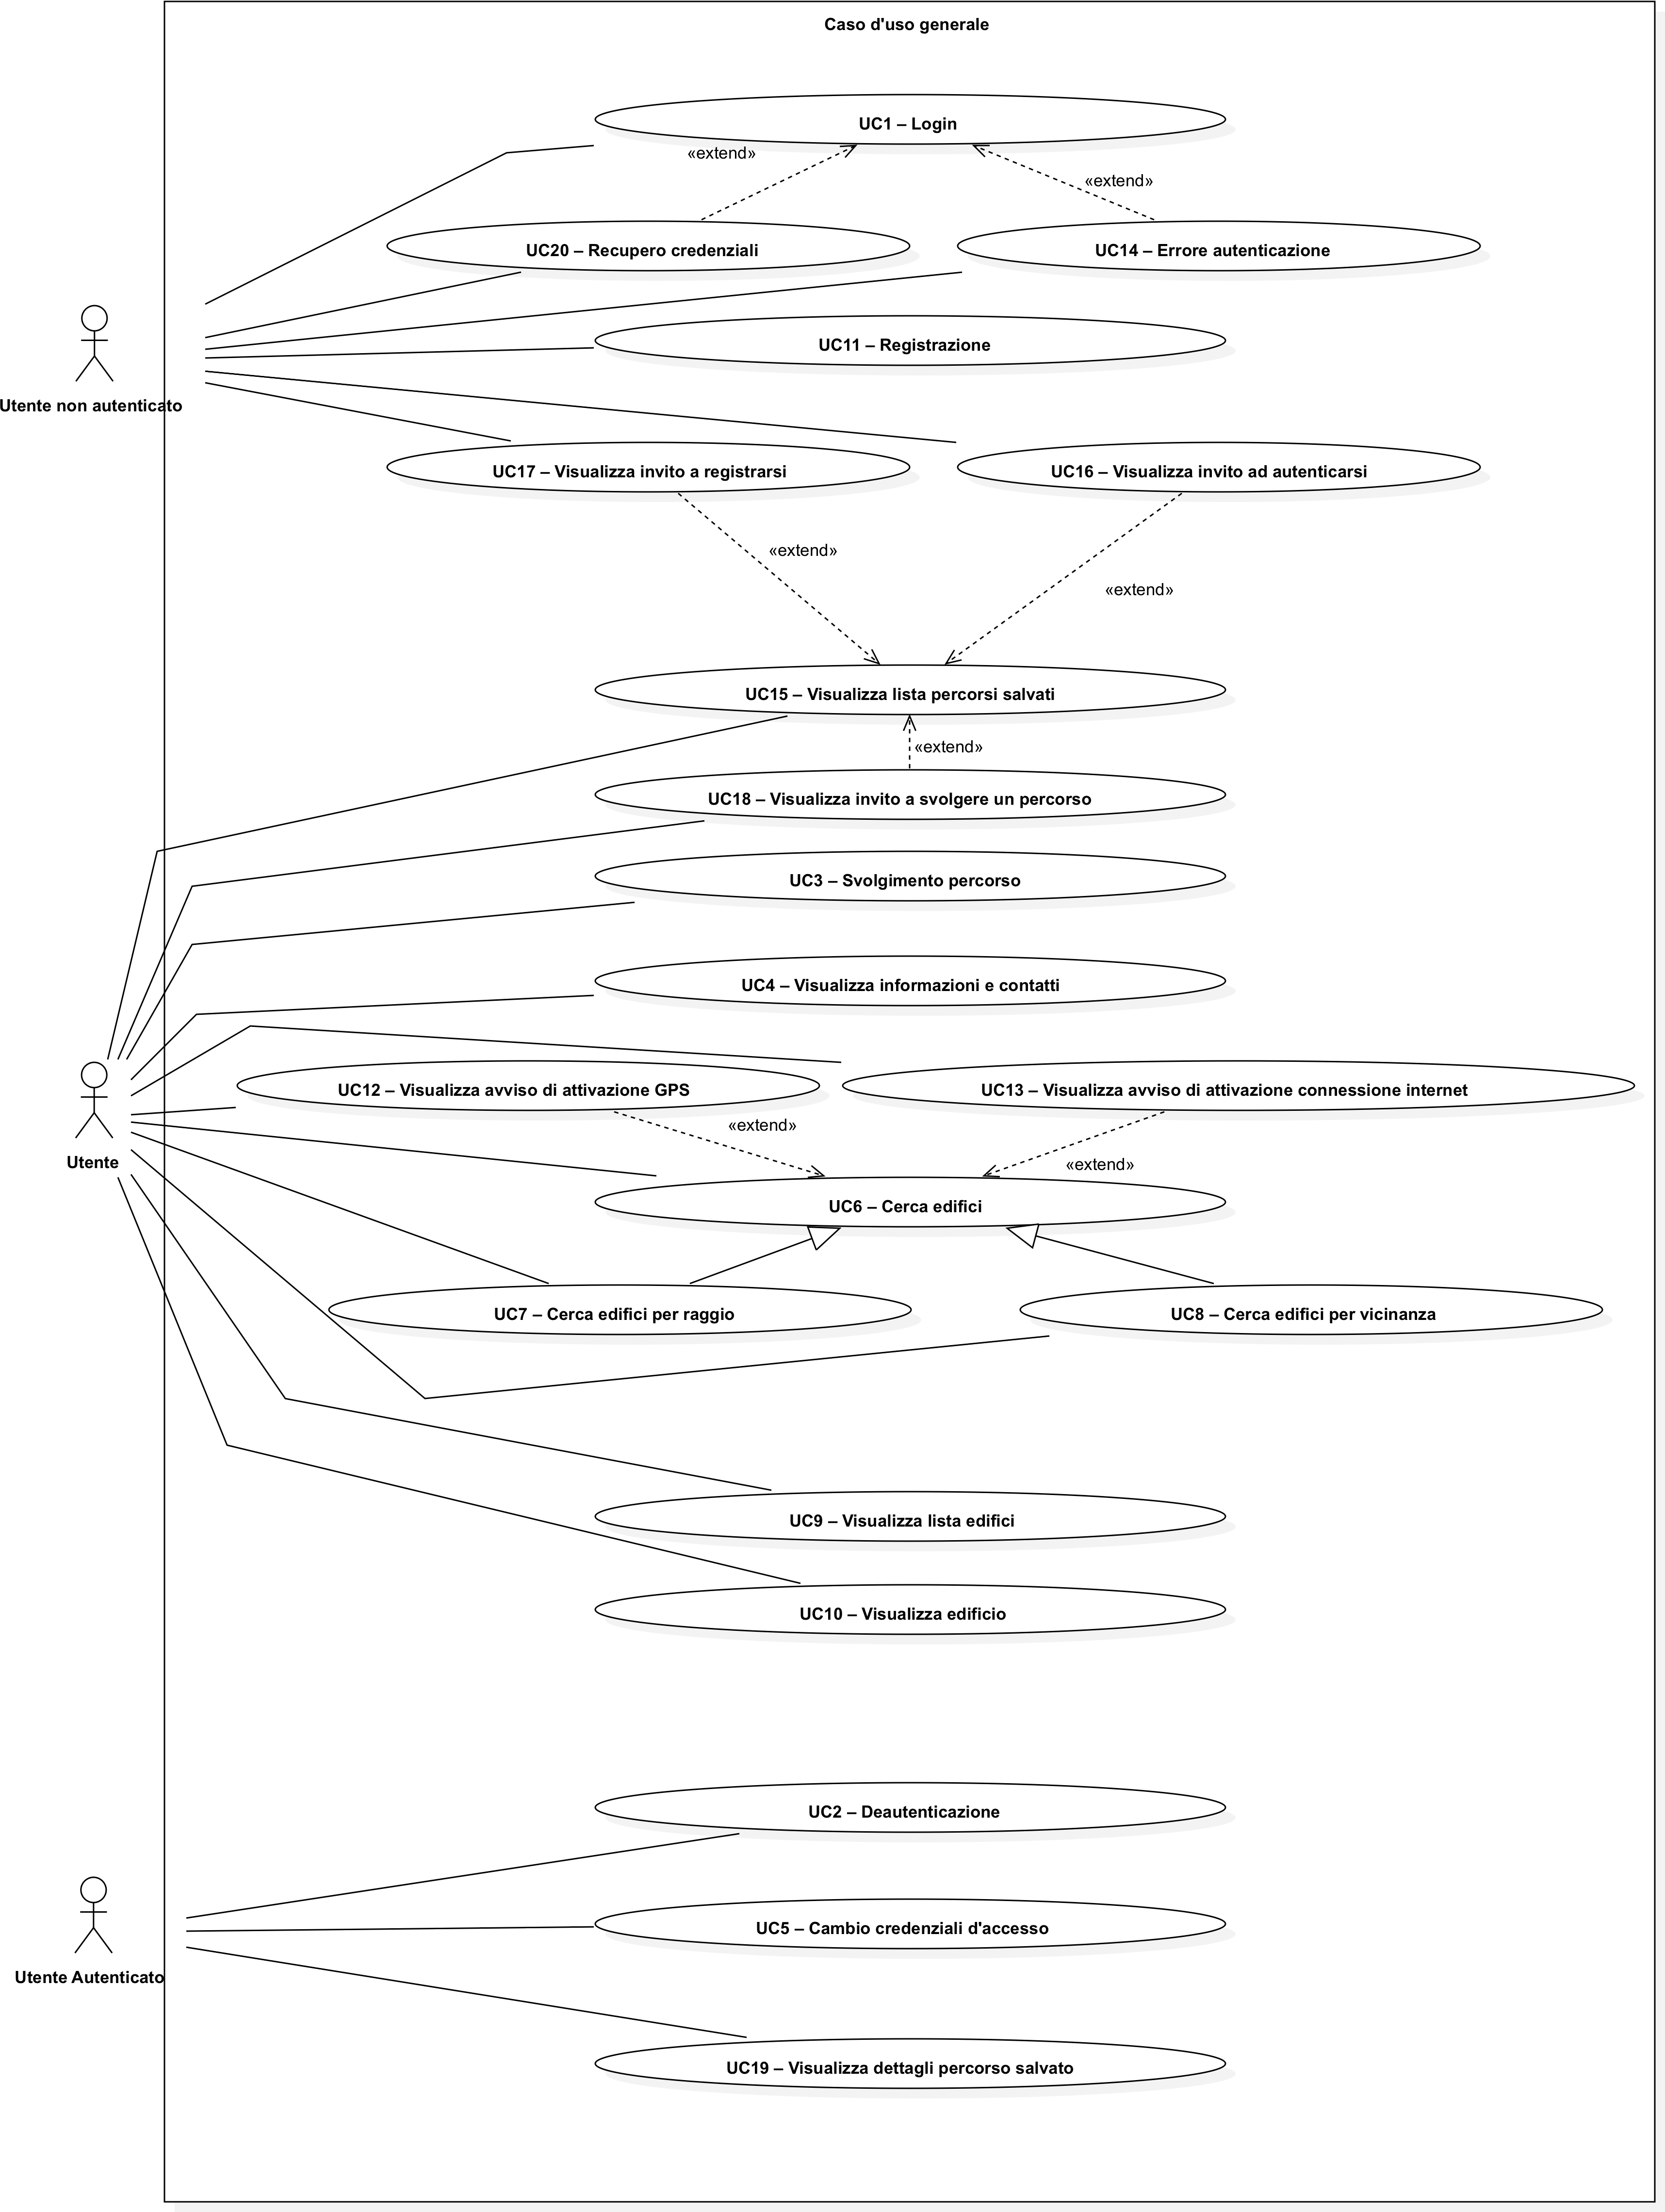
\includegraphics[scale=0.12]{img/Generale.png}
\caption{Caso d'uso Generale}
\end{figure}
